\begin{figure}[!htb]

    \centering

    \begin{subfigure}[b]{0.49\textwidth}
        \centering
        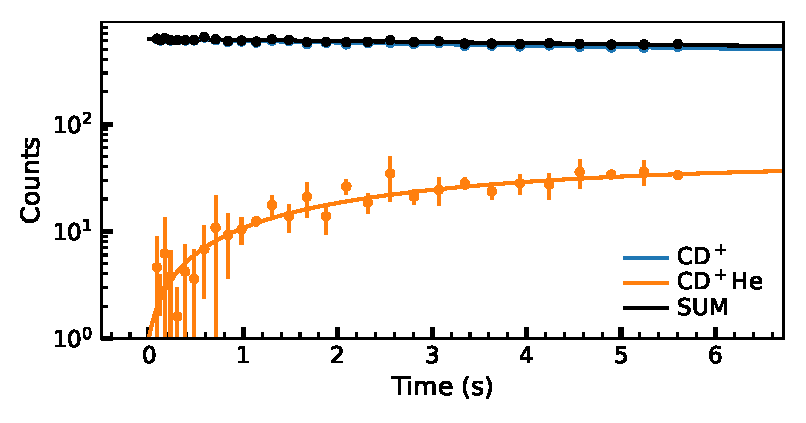
\includegraphics[width=1\textwidth]{figures/measurements/kinetics/off_kinetics_1.16_2e+14.pdf}
        \caption{}
        
    \end{subfigure}
    \hfill
    \begin{subfigure}[b]{0.49\textwidth}
        \centering
        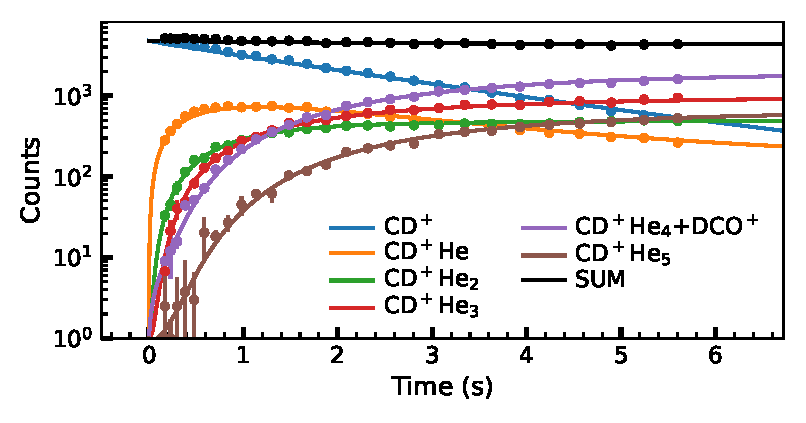
\includegraphics[width=1\textwidth]{figures/measurements/kinetics/off_kinetics_6.04_25e+14.pdf}
        \caption{}
        
    \end{subfigure}
    
    \caption{(a) and (b) shows the counts of primary and complex ions monitored as a function of trap time at  $ 1.16(2)\cdot10^{14}$~cm$^{-3}$ and  $6.0(2)\cdot10^{14}$~cm$^{-3}$ respectively at 4.8(3) K. The circle marker and the solid line represent measured and numerically fitted data, respectively.}
    \label{fig:fit:rate-constants}

\end{figure}